%************************************************
\chapter{ConfigurableSystems}\label{ch:configurableSystems}
%************************************************

\section{Configurable Systems}

Nearly, all modern software systems are configurable, there are multiple reasons for that. 
We want to give the user flexibility, by offering them to turn functionality on and off. 
In addition to that a configurable software system satisfies the demand of multiple user by offering a single software system that contains multiple features. 
\cite{TooManyKnobs}

\begin{figure}[h]
    \centering
    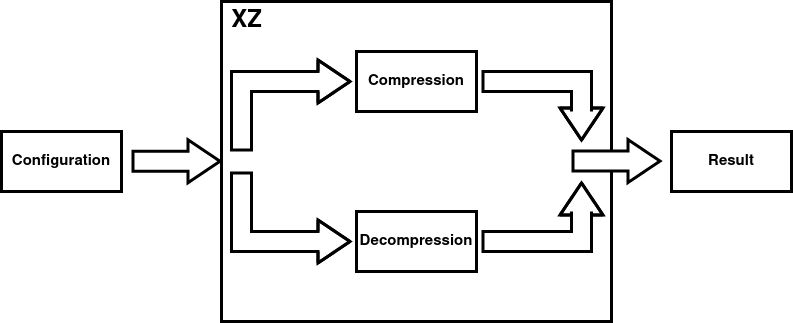
\includegraphics[scale=0.6]{gfx/ConfigurableSystemXZ.png}
    \caption{Scaled down verion xz}
    \label{fig:xz}
\end{figure}

As a example let us inspect the compression tool xz  \footnote{https://linux.die.net/man/1/xz}. In Figure ref{fig:xz}
we can see a scaled down version of xz, which contains two main functions (In reality many more), encryption and decryption, it is up to the user to 
decide what he needs, but regardless his choice both funcitons are contained in a single software.
